%-------------------------------------------------------------------
\chapter{State of the Art}
\label{c:sota}
%-------------------------------------------------------------------

%-------------------------------------------------------------------
\section{Context, data, and the case for structured spatial models}
\label{sec:sota:context}
%-------------------------------------------------------------------

Modelling spatially organised biological systems has a long tradition in mathematical and computational biology. The spatial arrangement of cells and the local signals they exchange strongly affect form and function. For example, morphogen gradients govern cell fate during development~\cite{rogers2011morphogen}; stem-cell identity and niche behaviour depend on spatial context; and both cancer invasion and tissue regeneration are driven by local cell-cell and cell-environment interactions in spatially structured tissues~\cite{noble2022spatial,seferbekova2023spatial}. So any computational model that aims to capture these phenomena must represent space explicitly. It must also respect the constraint that no single agent has access to global state: each cell may use only information from its immediate neighbourhood.
Classical approaches fall into two broad categories:
\begin{enumerate}
  \item \emph{Continuum models}, which use partial differential equations (reaction-diffusion, mechanochemical formulations).
  \item \emph{Discrete agent-based models}, in which each cell obeys rules that depend on local context.
\end{enumerate}
The first type is tractable in simple geometries but scales poorly to highly heterogeneous, discrete cell populations. The second is flexible and widely used in tissue and cancer modelling, but the rules are usually hand-tuned or fitted via simulation-based inference (e.g.\ approximate Bayesian computation~\cite{beaumont2002abc,sisson2018abc}). Learning such rules directly from high-dimensional observational data remains challenging. A central question in recent work is therefore how to combine spatial, local interaction with the ability to \emph{learn} dynamics from data using gradient-based optimisation \cite{mnca_milite2025}.

The data used to train or validate such models are diverse. In developmental biology and morphogenesis, target data may be static patterns (e.g.\ a desired shape or cell-type map) or temporal sequences of spatial configurations from time-lapse imaging or lineage tracing. In tissue and cancer modelling, researchers often use high-throughput microscopy, spatial transcriptomics, and synthetic data from stochastic simulators (e.g.\ stem-cell-driven growth and differentiation on a grid). In all cases, observations are high-dimensional (many cells, time points, or channels), and the underlying transition rules are unknown or only partly known. The goal is not only to fit the data but to obtain a \emph{mechanistic}, generative representation. Such a model can be run from new initial conditions, examined (e.g.\ to see which local rule applies where), and potentially steered by changing rules or initial state. This pushes the goal beyond pure prediction toward interpretable, generative spatial dynamics \cite{mnca_milite2025,nca_mordvintsev2020}.

An alternative is to use generic deep learning: for instance, convolutional or recurrent networks that map the current grid state (or a sequence of states) to the next state or to a target output. Such architectures have been used successfully for image-to-image prediction and video forecasting. However, they do not enforce locality by design. The effective receptive field of a deep convolutional network can span the entire grid, and how information propagates in space and time is encoded implicitly in the weights. There is no direct link to the biological assumption that cells communicate only with neighbours. In practice, long-horizon rollouts from these models often drift, diverge, or become unstable, especially when training data are limited or when the task requires extrapolation beyond the training distribution. Also, the learned dynamics are hard to interpret: one cannot easily extract a local rule or see which cells influence which. By contrast, cellular automata and their neural extensions assume that the next state of a cell depends only on a bounded neighbourhood. This bias restricts the hypothesis space, can improve sample efficiency when data are scarce, and yields models that match the mechanistic, agent-based view of biology used in much of the spatial modelling literature. The trade-off is less expressive power in exchange for interpretability, stability under rollout, and a parameterisation that fits the domain. The rest of this chapter surveys the literature along this line, from classical CA to neural and mixture-based CA, and places the model used in this thesis in a clear methodological and applied context.

%-------------------------------------------------------------------
\section{Cellular Automata}
\label{sec:sota:ca}
%-------------------------------------------------------------------

Cellular automata (CA) have been studied since the pioneering work of von Neumann on self-reproducing automata \cite{ca_vonneumann1966} and have since become a canonical framework for studying emergence from local rules; for a modern treatment see \cite{ca_hawkins2024}. A CA consists of a discrete grid of cells, each endowed with a state drawn from a finite (or, in continuous variants, real-valued) set. Time advances in discrete steps; at each step, every cell is updated according to a fixed rule that depends only on its own state and the states of the cells in a small neighbourhood. There is no central controller: the next configuration is determined solely by applying the same local rule everywhere in parallel. This formulation captures the essence of decentralised, spatially local computation and has been applied across physics, ecology, and biology; optimisation of CA rules via evolutionary curriculum strategies has also been explored \cite{ca_antal2021}.

Formally, let \(\mathcal{L}\) denote the set of cell positions (e.g.\ a finite or infinite subset of \(\mathbb{Z}^2\)), and \(\mathcal{S}\) the set of possible cell states. The neighbourhood of a cell at \((i,j)\) is a set \(\mathcal{N}(i,j) \subseteq \mathcal{L}\) of nearby positions (e.g.\ those within Chebyshev distance \(r\) for some radius \(r\)). The global state at time \(t\) is a function \(x_t : \mathcal{L} \to \mathcal{S}\). The update rule is a function \(\phi\) that maps the state of a cell and its neighbourhood to a new state:
\begin{equation}
x_{t+1}(i,j) = \phi\bigl( x_t(i,j), \, \{ x_t(i',j') : (i',j') \in \mathcal{N}(i,j) \} \bigr).
\end{equation}
The dynamics are fully specified by \(\phi\) and the initial condition \(x_0\). Despite this simplicity, CAs are known to exhibit a wide range of behaviours (from static or periodic patterns to chaos, self-replication, and universal computation) and have been the subject of extensive theoretical and applied work. In the biological context, the emphasis on locality and discreteness aligns with the view that cells interact primarily with nearby cells and that developmental and tissue-level dynamics can be approximated by discrete-time updates. CAs have accordingly been used as tools for simulating growth, pattern formation, and morphogenesis in the literature \cite{ca_vonneumann1966}. See \cref{fig:sota:ca_example} for an illustration.

\begin{figure}[t]
  \centering
  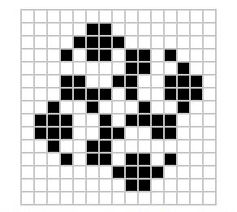
\includegraphics[width=0.62\textwidth]{figs/sota_ca_example}
  \caption{Example of a cellular automaton. \textbf{Legend:} discrete grid; each cell updated by a local rule~\cite{ca_vonneumann1966}.}
  \label{fig:sota:ca_example}
\end{figure}

The main limitation here is that the rule \(\phi\) is fixed and hand-crafted. Inverse design (finding a \(\phi\) that produces a desired global behaviour, e.g.\ a specific shape or regenerative response, from a simple seed) is difficult. Reverse-engineering such rules for biologically plausible outcomes is still an open problem. This has led to work where the update rule is \emph{learned} from data instead of being set in advance, i.e.\ to the neural cellular automata discussed in the next section.

%-------------------------------------------------------------------
\section{Neural Cellular Automata}
\label{sec:sota:nca}
%-------------------------------------------------------------------

Gilpin showed that CA update rules can be expressed as convolutional neural networks \cite{ca_gilpin2019}. Mordvintsev et al.\ then showed that such rules can be \emph{learned} from data via gradient-based optimisation, leading to what is now called Neural Cellular Automata (NCA) \cite{nca_mordvintsev2020}. NCAs keep the spatial structure and locality of classical CAs but replace the hand-crafted rule \(\phi\) with a function implemented by a small neural network. The same network is applied at every cell; only the local perception (and, in some extensions, a small amount of global conditioning) varies across the grid. Formally, NCAs replace \(\phi\) in the classical CA update with a learned map \(f_\theta\) that takes a local view of the grid and outputs an update (typically an increment) to the cell state.

A common formulation is
\begin{equation}
x_{t+1} = x_t + f_\theta\bigl( \mathcal{P}(x_t) \bigr),
\end{equation}
where \(\mathcal{P}(x_t)\) denotes a \emph{perception} step that, for each cell, aggregates information from a neighbourhood (e.g.\ the cell's own state plus gradient-like features in the horizontal and vertical directions, as in the Growing NCA model below). The network \(f_\theta\) is typically a shallow stack of \(1\times 1\) convolutions and nonlinearities, so that it operates in a local fashion and can be applied in one pass over the grid. Training is usually performed by minimising a loss between the state produced after a number of steps and a target (e.g.\ an image or a temporal trajectory), using backpropagation through time (BPTT)~\cite{werbos1990backpropagation,goodfellow2016deep}. Subsequent work has extended NCAs to texture synthesis, 3D morphogenesis, and classification tasks, and has explored variants with attention mechanisms, graph-based neighbourhoods, and Hamiltonian-inspired conservative dynamics~\cite{hnn_ca_greydanus2021}; the core idea of a single, learned local rule applied everywhere remains central \cite{nca_mordvintsev2020}, and recent work has examined both interpretability of the learned rules and their application to biological systems \cite{nca_bodnar2022,nca_randall2023}.

This shift from fixed to learned rules has several consequences that are relevant to the present thesis. First, NCAs can be trained to reproduce complex target dynamics (morphogenesis, texture synthesis, regeneration) without explicitly programming the transition rule. Second, the model remains interpretable in the sense that behaviour is driven exclusively by local updates. Third, the framework is differentiable end-to-end, so objectives can be defined at the level of global outcomes (e.g.\ match a target pattern) and the local rule can be optimised accordingly. For these reasons, NCAs have been adopted as a natural tool for modelling biological and self-organising systems where the goal is to learn growth and patterning from data rather than to postulate a specific \(\phi\) \cite{nca_mordvintsev2020}. \Cref{fig:sota:nca_schema} illustrates the generic NCA step.

\begin{figure}[t]
  \centering
  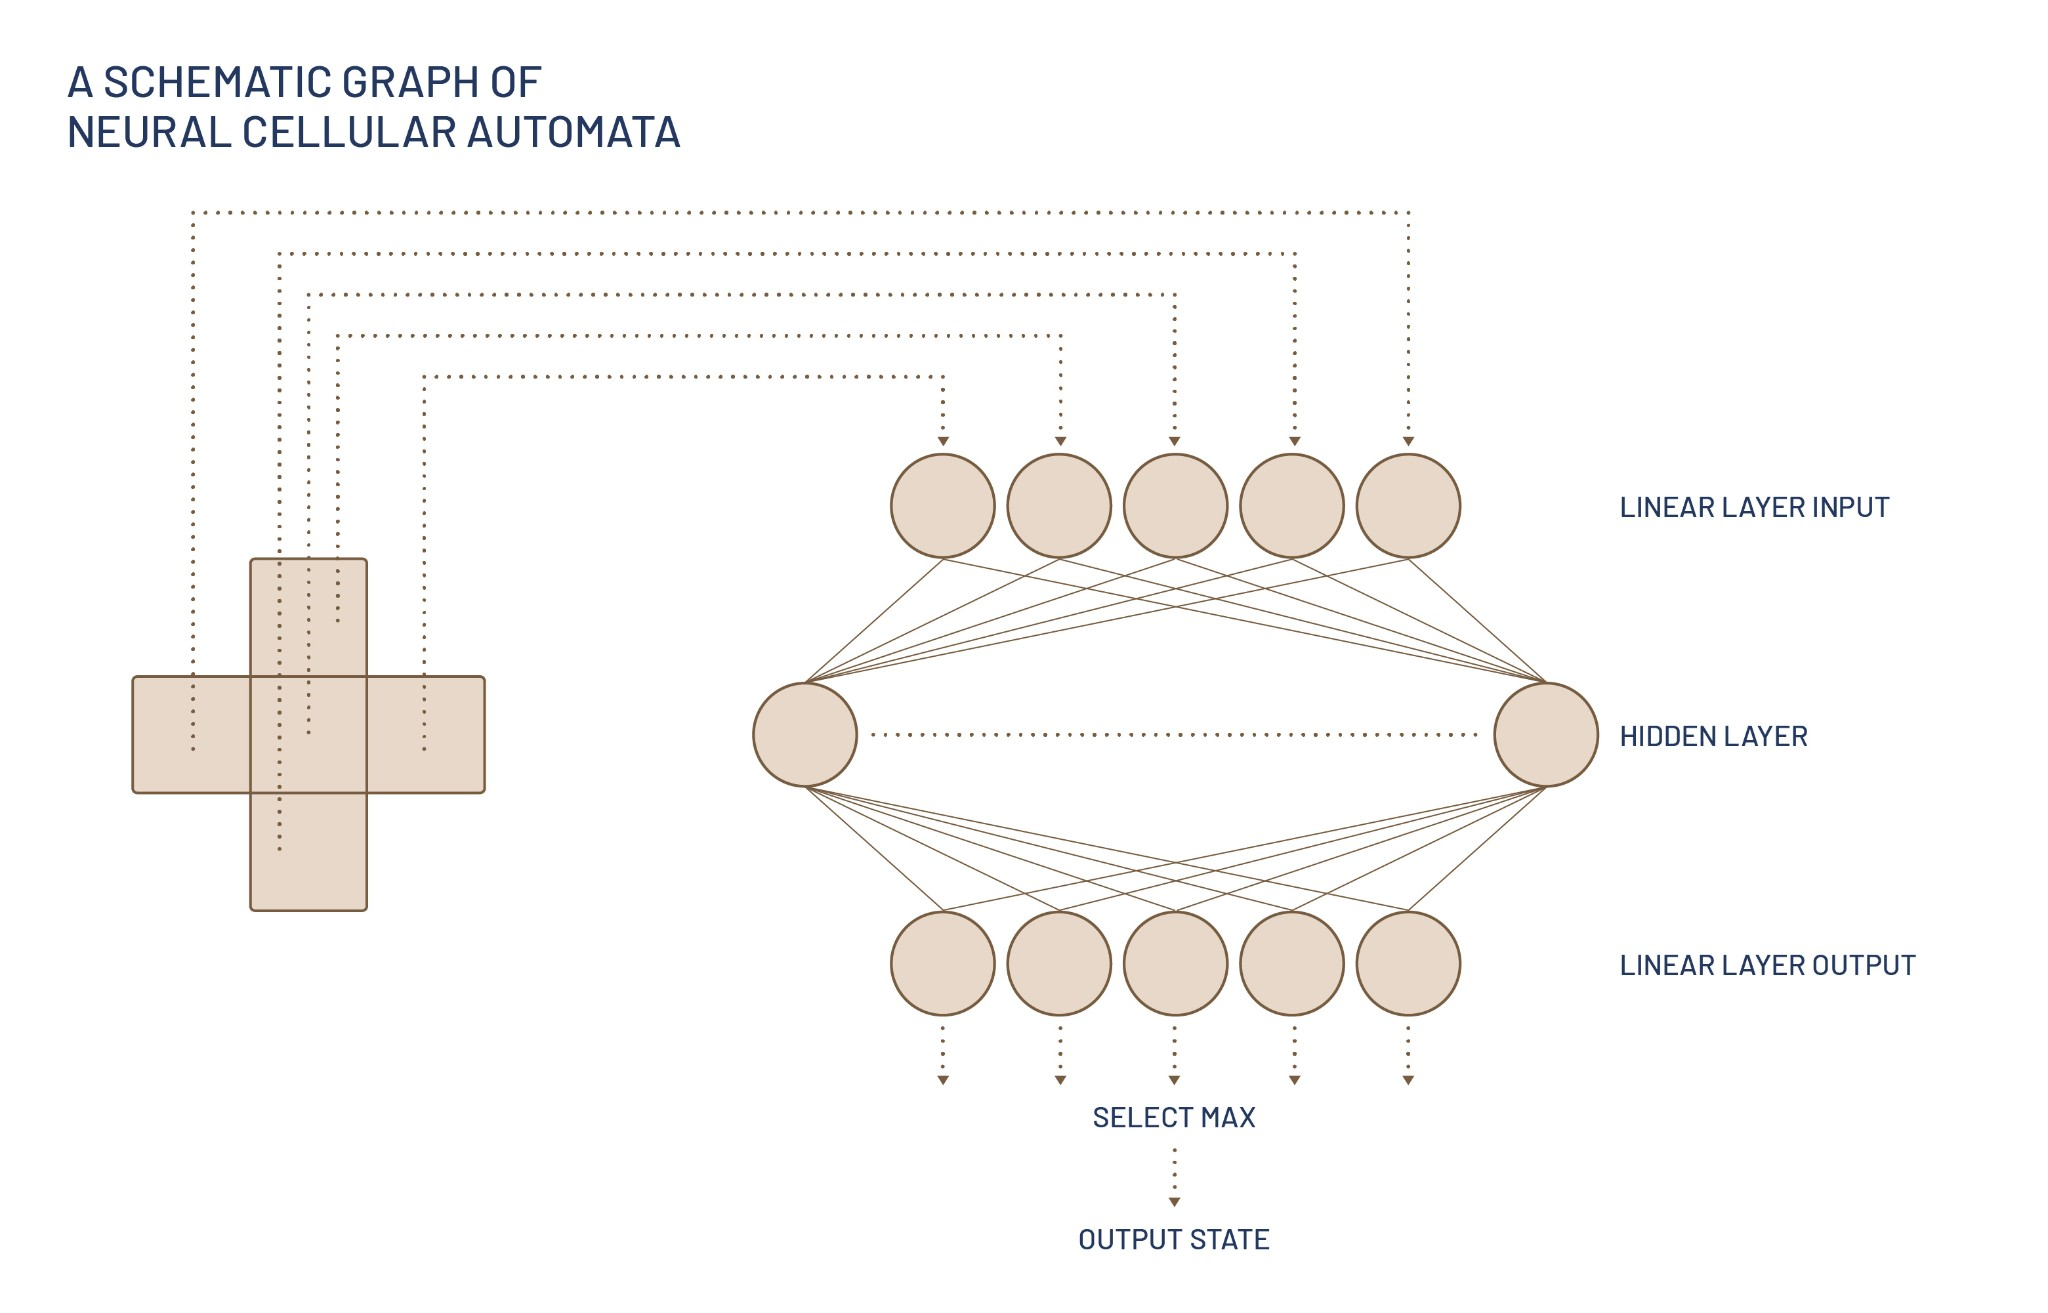
\includegraphics[width=0.72\textwidth]{figs/sota_nca_schema}
  \caption{Single NCA update step. \textbf{Legend:} perception (state and gradients) \(\rightarrow\) neural network \(\rightarrow\) state increment (applied residually). Adapted from Mordvintsev et al.~\cite{nca_mordvintsev2020}.}
  \label{fig:sota:nca_schema}
\end{figure}

%-------------------------------------------------------------------
\section{Growing Neural Cellular Automata}
\label{sec:sota:growing}
%-------------------------------------------------------------------

Mordvintsev et al.\ introduced \emph{Growing Neural Cellular Automata} in a setting that focuses explicitly on morphogenesis: the NCA is trained to grow a predefined multicellular pattern on a 2D grid from a single seed cell \cite{nca_mordvintsev2020}. This setting has since served as a reference benchmark and as a bridge between abstract NCA and biologically inspired notions of growth, stability, and regeneration.

\subsection{Cell state and perception}

Each cell is represented by a vector of 16 real values. The first three channels are RGB (the visible phenotype); the fourth is an alpha channel used to distinguish ``living'' cells (alpha \(> 0.1\)) from empty ones. The remaining channels are latent and used by the rule for internal signalling. Cells with no living neighbour in their \(3\times 3\) neighbourhood have their state set to zero at each step, so that only the pattern and its immediate frontier participate in the dynamics.

Perception is implemented by augmenting the cell state with local gradient information. Convolving the grid with Sobel filters~\cite{sobel1968isotropic} in the \(x\) and \(y\) directions yields, for each channel, estimates of \(\partial/\partial x\) and \(\partial/\partial y\)~\cite{szeliski2022computer}. The perception vector for a cell is the concatenation of its state, the gradients in \(x\), and the gradients in \(y\), giving a \(16 \times 3 = 48\)-dimensional input per cell. This design reflects the idea that cells in real morphogenesis often rely on chemical or electrical gradients to coordinate; the Sobel filters provide a fixed, differentiable way to sense direction and rate of change.

\subsection{Update rule and stochasticity}

The update rule is a small fully connected (or equivalently \(1\times 1\) convolutional) network that maps the 48-dimensional perception to a 16-dimensional state increment. The final layer is initialised to zero so that the initial behaviour is close to ``do nothing'', and no ReLU is applied to the output so that updates can be positive or negative. The state is updated in a residual fashion: \(x_{t+1} = x_t + \Delta x_t\). \Cref{fig:sota:growing_update} summarises one full update step (perception, update, stochastic mask, alive masking).

To relax the assumption of a global synchronous clock, the model applies a random per-cell mask to the update: with probability 0.5 (during training), the update at a cell is zeroed. Thus cells effectively update at random times, which can improve robustness and is closer to asynchronous biological update.

\begin{figure}[t]
  \centering
  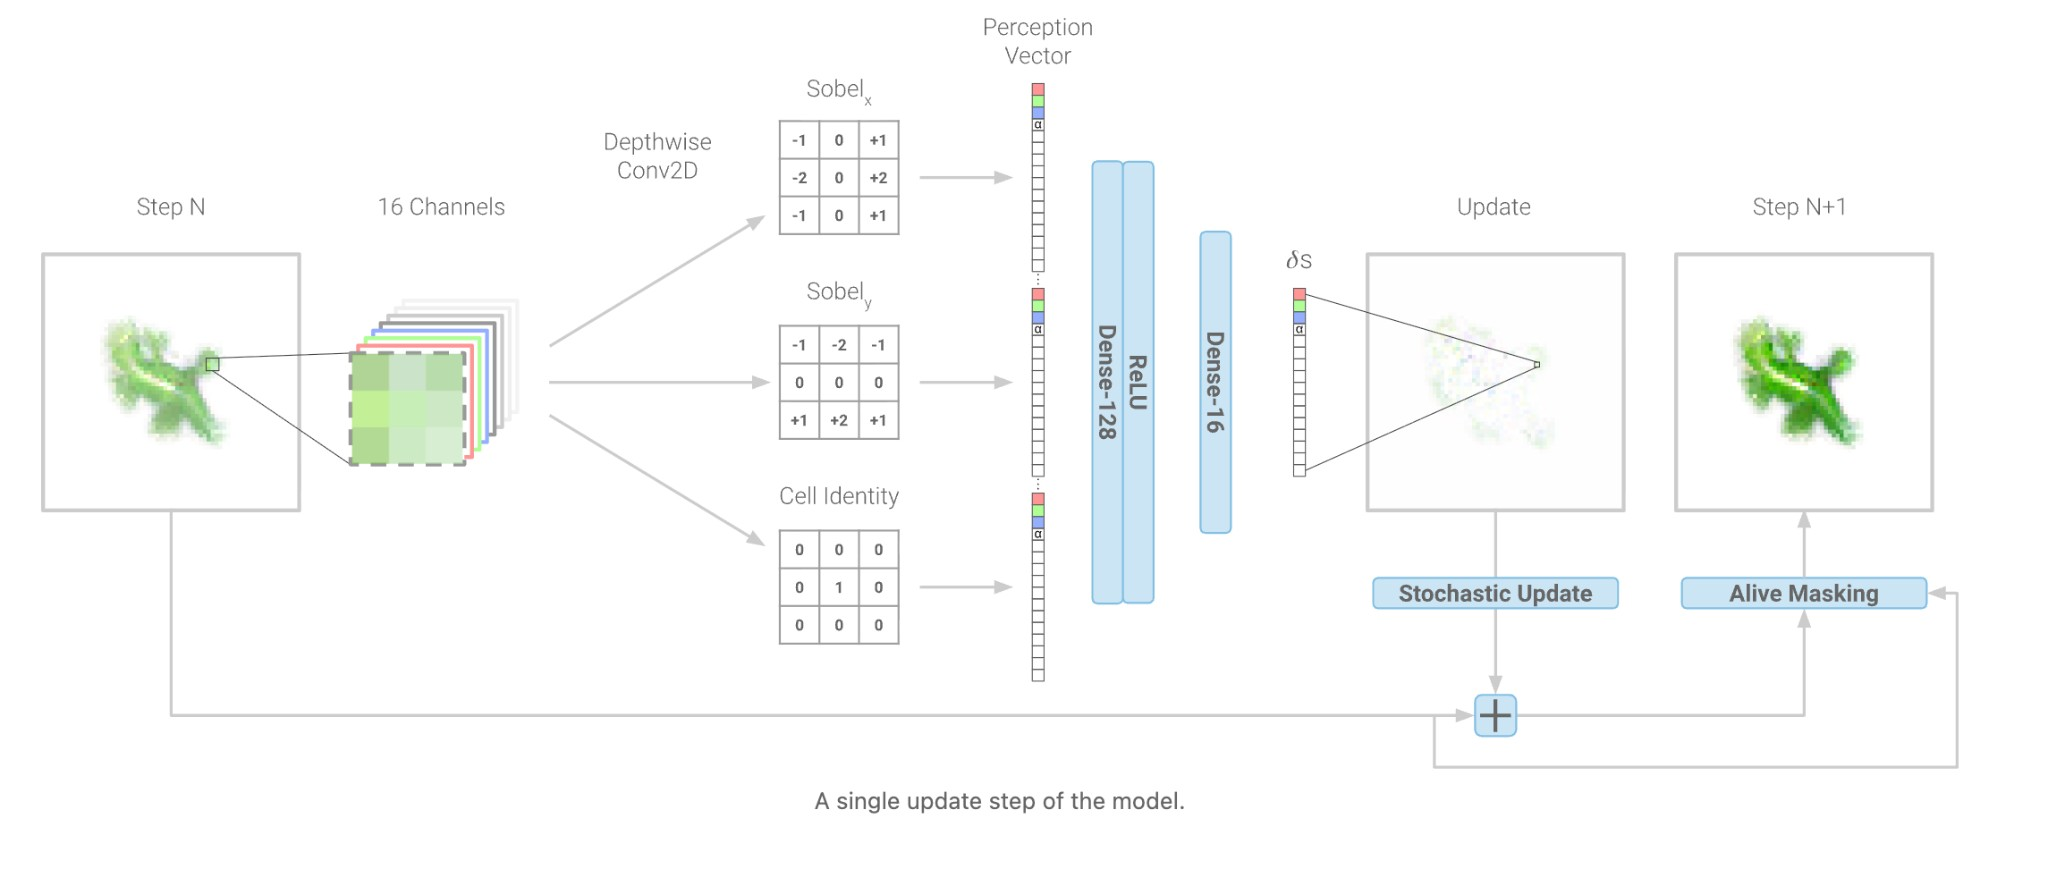
\includegraphics[width=0.76\textwidth]{figs/sota_growing_update}
  \caption{One update step of the Growing NCA. \textbf{Legend:} perception (state + gradient channels) \(\rightarrow\) update network \(\rightarrow\) stochastic mask \(\rightarrow\) alive masking. Adapted from Mordvintsev et al.~\cite{nca_mordvintsev2020}.}
  \label{fig:sota:growing_update}
\end{figure}

\subsection{Training for growth, persistence, and regeneration}

Training proceeds in three phases \cite{nca_mordvintsev2020}. In the first, the CA is trained to reach a target pattern from a single seed after a random number of steps in a fixed range; the loss is pixel-wise L2 between the final state and the target. This yields growth but often unstable long-term behaviour (patterns may explode or decay). In the second phase, a \emph{sample pool} of states is maintained: at each training step, a batch is sampled from the pool, the highest-loss sample is replaced by the seed, and the model is run on the batch; the resulting states are written back into the pool. The dynamics are thus trained not only to grow from the seed but also to persist and to correct from states that are already close to or far from the target, encouraging the target to become an attractor in the dynamical-systems sense (a configuration toward which trajectories converge and remain). In the third phase, a subset of the pool samples is \emph{damaged} (e.g.\ by zeroing a random circular region) before iteration, so that the model must learn to regenerate. Models trained with this damage regime exhibit substantially stronger regenerative behaviour than those trained only for growth or persistence \cite{nca_mordvintsev2020}. \Cref{fig:sota:growing_training_steps} shows the evolution of a pattern during training; \cref{fig:sota:growing_pool} and \cref{fig:sota:growing_regeneration} illustrate pool-based training and regeneration.

\begin{figure}[t]
  \centering
  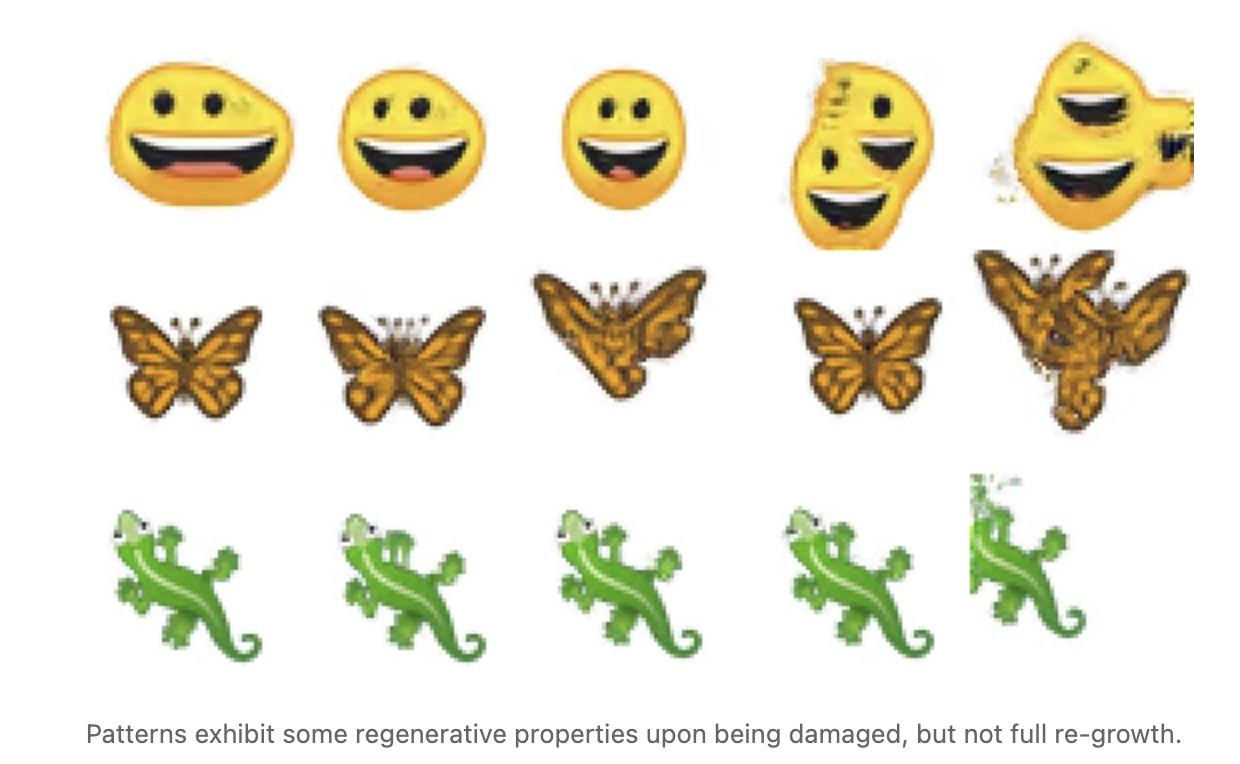
\includegraphics[width=0.72\textwidth]{figs/sota_growing_training_steps}
  \caption{CA behaviour at training steps 100, 500, 1000, 4000. \textbf{Legend:} columns = training step; pattern evolves from initial seed toward target. Adapted from Mordvintsev et al.~\cite{nca_mordvintsev2020}.}
  \label{fig:sota:growing_training_steps}
\end{figure}

\begin{figure}[t]
  \centering
  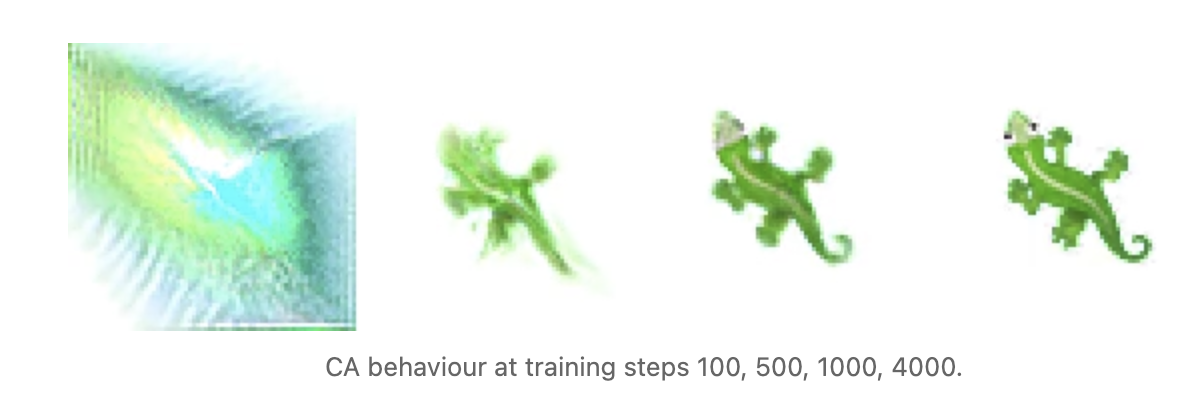
\includegraphics[width=0.72\textwidth]{figs/sota_growing_pool}
  \caption{Sample-pool training. \textbf{Legend:} random sample of patterns in the pool during training. Adapted from Mordvintsev et al.~\cite{nca_mordvintsev2020}.}
  \label{fig:sota:growing_pool}
\end{figure}

\begin{figure}[t]
  \centering
  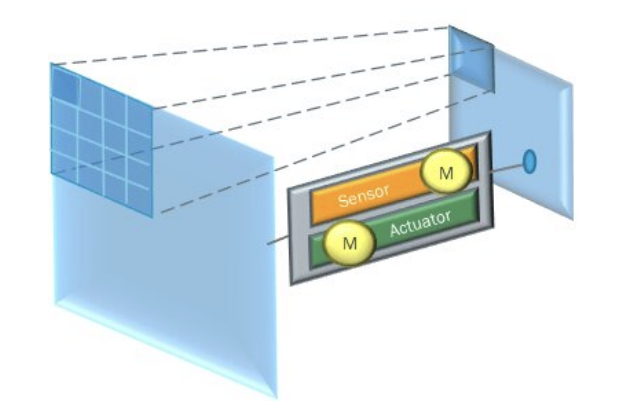
\includegraphics[width=0.72\textwidth]{figs/sota_growing_regeneration}
  \caption{Regeneration. \textbf{Legend:} pattern damaged then iterated; extent of recovery shown. Adapted from Mordvintsev et al.~\cite{nca_mordvintsev2020}.}
  \label{fig:sota:growing_regeneration}
\end{figure}

This progression (growth, persistence, regeneration) demonstrates that a single local rule, learned with appropriate objectives and data diversity, can capture morphogenetic and homeostatic behaviour. It also motivates the next step in the literature: the introduction of multiple rules and explicit stochasticity to better match the variability and heterogeneity of real biological systems.

%-------------------------------------------------------------------
\section{Limits of Standard NCA and the Role of Stochasticity}
\label{sec:sota:limits}
%-------------------------------------------------------------------

Standard NCA models, including the Growing NCA described above, are deterministic: given the same initial state and the same (possibly stochastic) update mask, the trajectory is uniquely determined. It is well established in the biological literature that real systems are inherently stochastic: gene expression, cell division, and differentiation are subject to molecular noise; genetically identical cells can follow different fates; and tissue-level outcomes emerge from the statistics of many such noisy, local events. Deterministic NCAs can at best produce a single ``average'' trajectory and do not naturally represent variability across runs or the possibility that different cells might follow different behavioural programmes.

Furthermore, in real morphogenesis and tissue maintenance, cells are not all executing the same programme: they differentiate into distinct types and adopt different roles. A single global update rule can encode complex behaviour through the hidden state, but it does not explicitly represent a \emph{mixture} of distinct local behaviours (e.g.\ one rule favouring proliferation at the border, another maintaining quiescence in the interior). These observations have motivated a line of work that extends the NCA framework to support multiple update rules and stochastic selection among them, so that both spatial heterogeneity (different rules in different regions) and variability across realisations can be captured. The Mixture of Neural Cellular Automata (MNCA) framework, reviewed in the next section, implements this extension \cite{mnca_milite2025}.

%-------------------------------------------------------------------
\section{Mixture of Neural Cellular Automata}
\label{sec:sota:mnca}
%-------------------------------------------------------------------

Milite et al.\ \cite{mnca_milite2025} introduced the Mixture of Neural Cellular Automata (MNCA), a framework that addresses two limitations of standard NCAs: their deterministic nature, which poorly matches the stochasticity of real biological systems (e.g.\ gene expression, cell differentiation, carcinogenesis), and the lack of an explicit representation of heterogeneous local behaviours. By combining mixture models with the NCA paradigm, MNCA allows each cell to be governed by one of \(K\) distinct neural update rules, with the choice made probabilistically from the current state. The authors further propose an extension with \emph{intrinsic noise}: a Gaussian latent vector fed into each rule so that even the same rule can produce stochastic updates, thereby capturing intra-cluster variability. The result is a stochastic, spatially heterogeneous dynamics that can be trained end-to-end and that offers interpretable rule assignments for post-hoc analysis \cite{mnca_milite2025}. MNCA constitutes the central model used in this thesis; all experiments reported in \cref{c:implementation} and \cref{c:results} are based on it.

\subsection{Formal definition and two variants}

Consider a grid of cells; let \(s^t_i \in \mathcal{S}\) denote the state of cell \(i\) at time \(t\) and \(\mathcal{N}(i)\) its neighbourhood. The authors define \(K\) neural transition functions \(\phi_k(\cdot; \theta_k)\), each mapping the local configuration (cell state and neighbours) to a state increment. A \emph{rule selector} is a neural network \(\pi(\cdot; \eta)\) that, given the current cell state (and optionally noise), outputs a \(K\)-dimensional probability vector over rules.

\paragraph{Mixture NCA (no intrinsic noise).} The rule index for cell \(i\) at time \(t\) is drawn from a Categorical distribution parametrised by \(\pi(s^t_i; \eta)\). Denoting by \(z \in \{1,\ldots,K\}\) the selected rule (one-hot encoded as \(z_k\)), the update is
\begin{equation}
z \sim \mathrm{Cat}\bigl(\pi(s^t_i; \eta)\bigr), \qquad
s^{t+1}_i = s^t_i + \sum_{k=1}^{K} z_k \, \phi_k\bigl(s^t_i, \{s^t_j : j \in \mathcal{N}(i)\}; \theta_k\bigr).
\end{equation}
Thus exactly one rule applies per cell per step; the Categorical is sampled so that the process is stochastic. To backpropagate through the discrete choice, the authors use the Gumbel-Softmax / Concrete trick~\cite{jang2017gumbel,maddison2017concrete,mnca_milite2025}.

\paragraph{MNCA with intrinsic noise.} Biological systems often exhibit variability even among cells that share the same ``type'' or context. To allow for intra-rule stochasticity, the update functions are given an extra input \(x_k \sim \mathcal{N}(0, I)\) sampled once per rule (or per cell and rule) and concatenated to the perception. The update becomes
\begin{equation}
z \sim \mathrm{Cat}\bigl(\pi(s^t_i; \eta)\bigr), \quad
x_k \sim \mathcal{N}(0, 1), \qquad
s^{t+1}_i = s^t_i + \sum_{k=1}^{K} z_k \, \phi_k\bigl(s^t_i, \{s^t_j : j \in \mathcal{N}(i)\}, x_k; \theta_k\bigr).
\end{equation}
The noise \(x_k\) is an internal source of randomness that the network can use to implement stochastic behaviour within each rule (e.g.\ random timing of division or differentiation). In the paper's experiments, both variants are evaluated; the one with intrinsic noise often yields better robustness and more realistic tissue statistics \cite{mnca_milite2025}.

\subsection{Architecture and implementation}

The paper keeps a simple, consistent architecture across tasks. Perception is the same as in many NCAs: the state is concatenated with its spatial gradients in \(x\) and \(y\) obtained via Sobel filters, i.e.\ \(\mathcal{P}(s) = \mathrm{cat}(s, \nabla_x s, \nabla_y s)\). Each rule \(\phi_k\) is implemented as two \(1\times 1\) convolutional layers: a hidden layer with ReLU on the perceived input (and, in the noisy variant, concatenated with \(x_k\)), then a linear layer that outputs the state increment. The rule selector \(\pi\) is a network of the same type but takes only the \emph{current cell state} \(s^t_i\) as input (not the full perception), so that the assignment depends on the cell's own state rather than on neighbour states. Training uses the mean squared error between the predicted and target state; optimisation is performed with Adam~\cite{kingma2014adam} and a multi-step learning-rate schedule, as is standard in deep learning~\cite{goodfellow2016deep}. Depending on the task, the update is applied as a residual (\(s^{t+1}_i = s^t_i + \Delta s\)) or the state is replaced entirely. Key hyperparameters (number of channels, number of rules \(K\), hidden dimension, residual or not) are reported per experiment: for example, the tissue-growth setup uses 6 channels, 5 rules, hidden dimension 128, and no residual update \cite{mnca_milite2025}. \Cref{fig:sota:mnca_schema} corresponds to Figure~1 in the paper, which summarises the full pipeline: spatial filters, central cell and neighbours, rule selector (MLP) yielding rule probabilities, and the selected NCA with optional noise injection.

\begin{figure}[t]
  \centering
  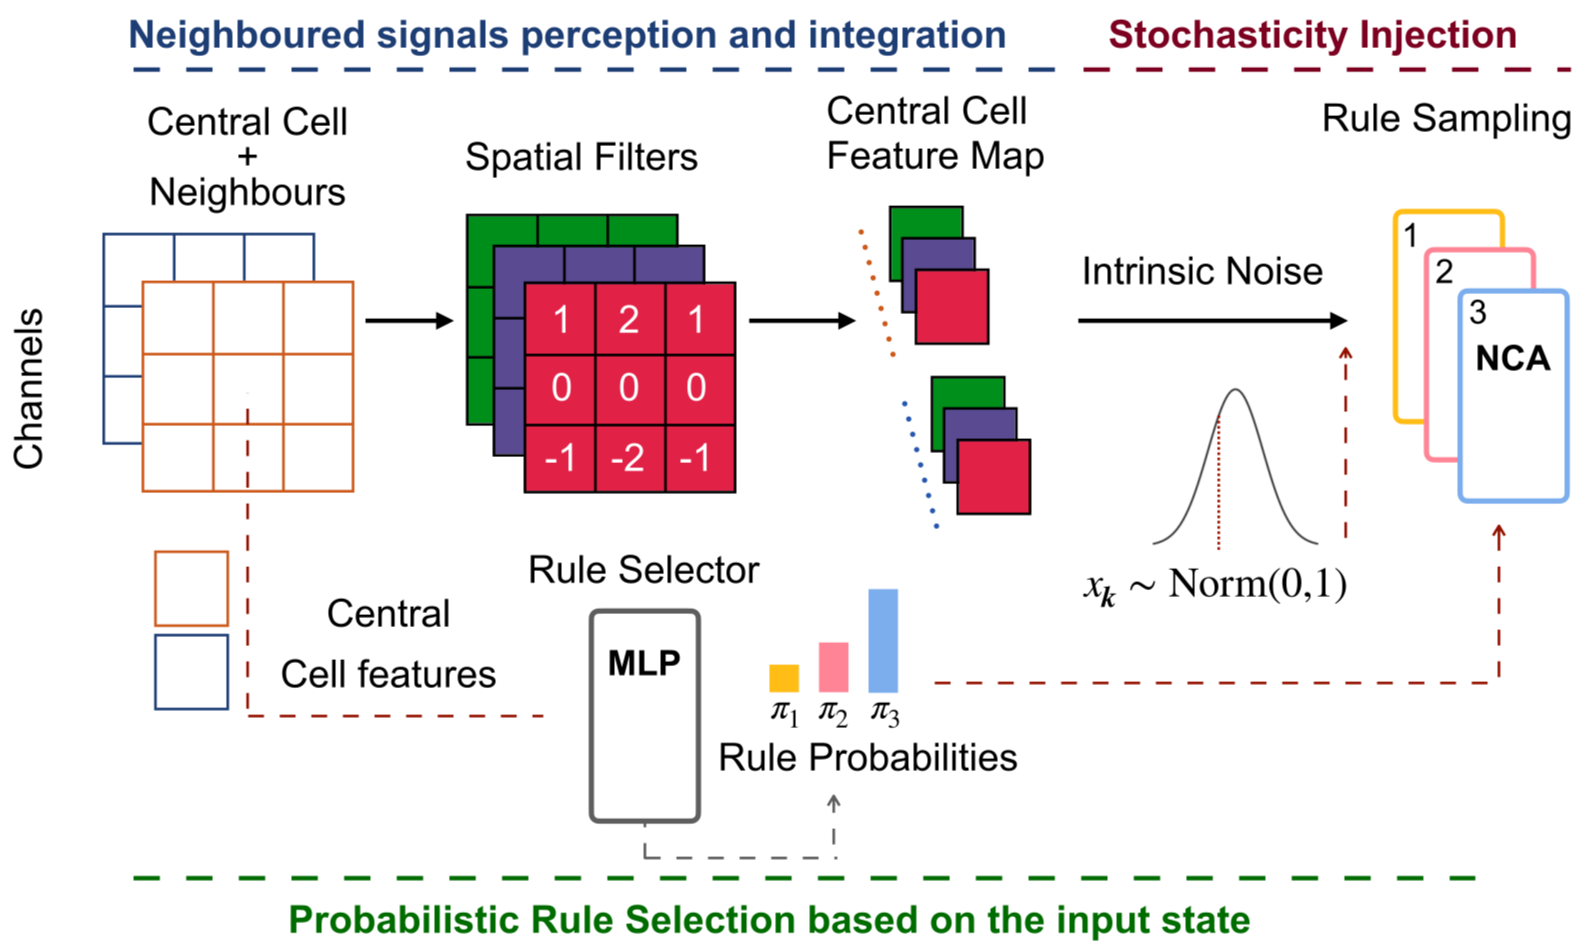
\includegraphics[width=0.76\textwidth]{figs/sota_mnca_schema}
  \caption{MNCA architecture. \textbf{Legend:} perception (central cell + neighbours) \(\rightarrow\) rule selector (MLP) \(\rightarrow\) rule probabilities; selected rule applied to perceived state; optional noise \(x_k\) for intrinsic-noise variant.}
  \label{fig:sota:mnca_schema}
\end{figure}

\subsection{Experimental evidence and interpretability}

The paper evaluates MNCA in three domains.
\begin{itemize}
  \item \textbf{Synthetic tissue growth and differentiation:} a stochastic simulator generates epithelial-like tissues with five cell types (stem, two intermediate, two differentiated) on a \(35\times 35\) grid from an initial cluster of stem cells. MNCA and MNCA with intrinsic noise are trained to reconstruct the state at each time step. They substantially outperform a deterministic NCA and a Gaussian NCA (GCA)~\cite{gnca_jeandelle2024} in terms of KL divergence of the cell-type distribution, Wasserstein distance on tissue size, and Wasserstein distance on border complexity, following recent practice in using Wasserstein-based metrics in machine learning~\cite{arjovsky2017wasserstein}. For example, the deterministic NCA reaches a KL divergence of about 2.06 while MNCA reaches about 0.02; the model with intrinsic noise further improves border fidelity \cite{mnca_milite2025}. Moreover, the learned rule assignments align with cell types: plotting the probability of each rule across the grid shows that roughly one rule is associated with each cell type (and one with empty space), with some rules shared (e.g.\ stem and one differentiated type), indicating that the model has discovered an interpretable partition of the state space.
  \item \textbf{Image morphogenesis:} the model is trained on emoji-like target images (as in Mordvintsev et al.) and then tested \emph{without} having seen perturbations during training. Under chunk removal, Gaussian noise addition, and sparse pixel removal, mixture-based NCAs recover the target image more reliably than the deterministic NCA; the error over recovery steps often peaks then decreases, suggesting that the target acts as an attractor. The GCA baseline does not show a clear advantage over the deterministic NCA in these experiments.
  \item \textbf{Unsupervised segmentation of microscopy images:} using high-content screening data (BBBC031v1), the authors initialise one seed per cell centroid and run the MNCA. The inferred rule assignments segment the tissue into regions that correlate with morphological and proteomic features (e.g.\ a provided ``cell shape parameter''), and constraining which rules are active at inference time can steer the population toward different phenotypes.
\end{itemize}
Together, these results support the claim that MNCA captures diverse local behaviours, improves robustness, and provides interpretable rule-based segmentation \cite{mnca_milite2025}.

\subsection{Motivations and advantages}

MNCA provides \emph{spatial heterogeneity}: different regions of the grid can specialise to different rules (e.g.\ by cell type or by position). It also provides \emph{temporal stochasticity} through both the random choice of rule and, in the noisy variant, the internal noise \(x_k\). This aligns with the view that biological cells exhibit context-dependent and inherently noisy behaviour. From a modelling perspective, the mixture can represent distinct behavioural programmes (proliferation, quiescence, differentiation) that are selected or mixed according to local state. From an interpretability perspective, the rule-assignment maps allow one to see how the model partitions the grid into functional regions and to relate those partitions to known biological or morphological structure. Finally, the explicit stochasticity and multiplicity of rules make MNCA a better fit for biological growth and self-organisation than a single deterministic NCA \cite{mnca_milite2025}. In this thesis we adopt MNCA as the base model and study how its behaviour changes when we vary the spatial neighbourhood size.

%-------------------------------------------------------------------
\section{Hierarchy in Self-Organising Systems and in NCA}
\label{sec:sota:hierarchy}
%-------------------------------------------------------------------

Biological systems are organised at multiple scales: cells form tissues, tissues form organs, and organs form organisms. Communication and control occur both within and across these scales. A single-scale NCA models dynamics at one level (e.g.\ cells on a grid) and does not explicitly represent higher-level structure (tissues, organs) or feedback from larger scales to smaller ones.

Hierarchical NCA (H-NCA) \cite{hnca_pande2023} addresses this by arranging several NCA modules in a hierarchy. Each cell of an NCA at a higher level is associated with a \emph{cluster} of cells of the NCA at the level below. The higher-level cell receives a summary of the state of its cluster (via a sensor) and can influence the lower-level NCA through signal channels (via an actuator). Training is phased: the lower-level NCA is trained toward its own goal; once it reaches a stable state, feedback is sent to the level above, which then modulates the lower level. This allows the system to exhibit multi-phase behaviour (e.g.\ growth then differentiation) and to model phenomena such as cell differentiation and metamorphosis, where the trigger for a new phase comes from within the system rather than from an external controller. The authors show that such hierarchical organisation can improve the capacity to evolve and maintain complex patterns and to coordinate behaviour across scales \cite{hnca_pande2023}. \Cref{fig:sota:hnca_arch} illustrates the H-NCA layout.

\begin{figure}[t]
  \centering
  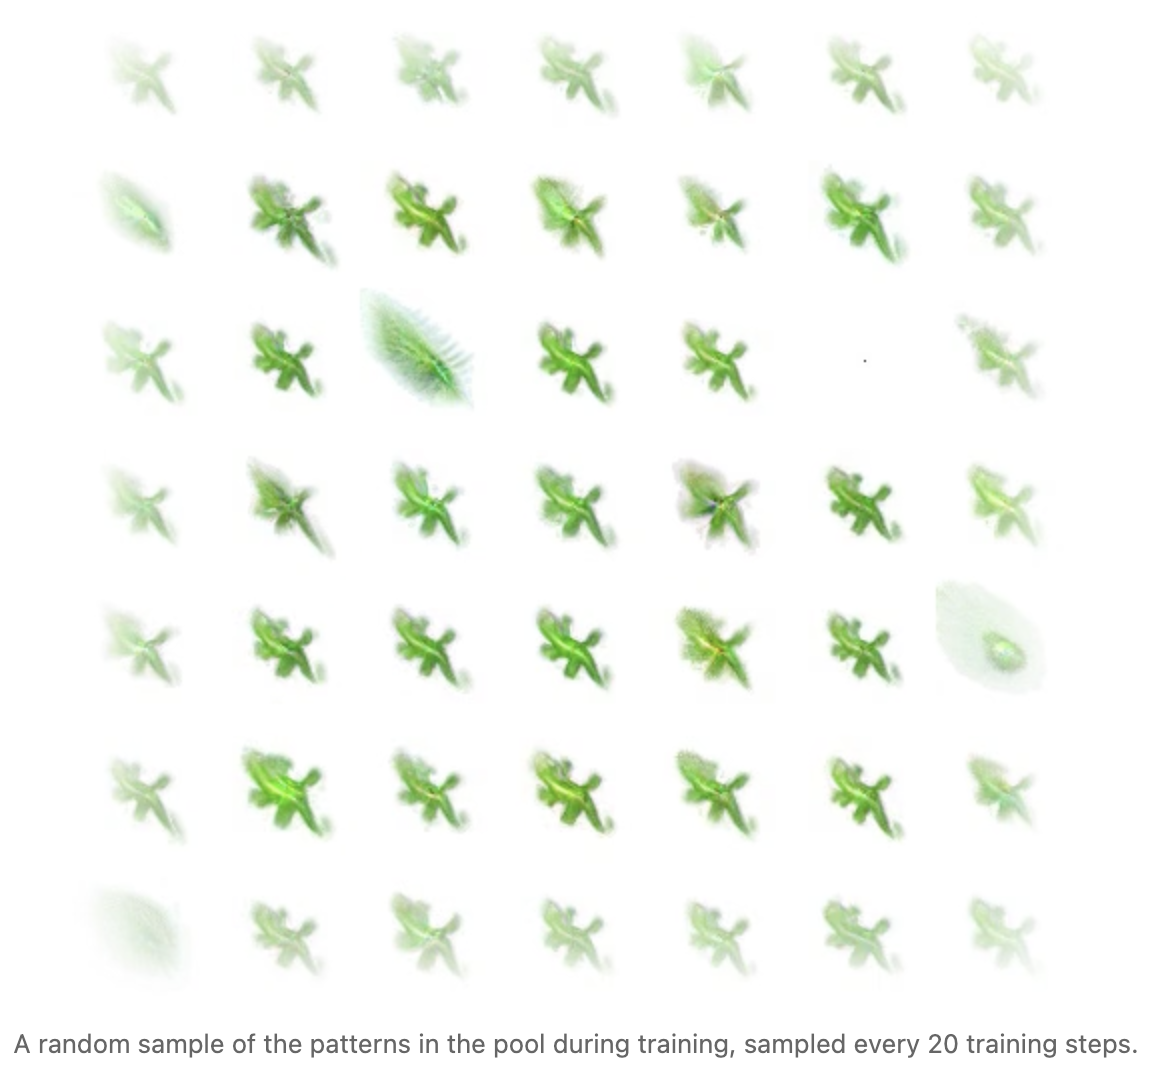
\includegraphics[width=0.72\textwidth]{figs/sota_hnca_architecture}
  \caption{H-NCA. \textbf{Legend:} parent NCA cells each control a cluster of child NCA cells; sensor (child\(\rightarrow\)parent) and actuator (parent\(\rightarrow\)child) mediate feedback. Adapted from Pande et al.~\cite{hnca_pande2023}.}
  \label{fig:sota:hnca_arch}
\end{figure}

Although hierarchical NCA is not directly used in the experiments of this thesis, it provides a broader perspective on the literature: the MNCA model adopted here operates at a single scale with multiple rules; future work could combine mixture-style stochasticity with hierarchical structure to capture both heterogeneity at one scale and coordination across scales.

%-------------------------------------------------------------------
%\section{Connections to Topological Deep Learning}
%\label{sec:sota:topological}
%-------------------------------------------------------------------

% (Discussion of topological deep learning moved to future work; see \cref{sec:conc:future}.)

%-------------------------------------------------------------------
\section{Synthesis and Positioning of This Thesis}
\label{sec:sota:synthesis}
%-------------------------------------------------------------------

In summary, the literature shows a clear progression. Classical cellular automata establish that local rules suffice for emergent global behaviour but leave the rule design to the modeller; inverse design remains difficult. Neural cellular automata address this by learning the rule from data while preserving locality and differentiability; the link between CA and convolutional networks was established by Gilpin \cite{ca_gilpin2019}, and learning from data for morphogenesis was demonstrated by Mordvintsev et al.\ \cite{nca_mordvintsev2020}. Growing NCA specialises the framework to growth from a seed and introduces training strategies (sample pool, damage) for persistence and regeneration. Standard NCA, however, remain deterministic and single-rule, which limits their ability to capture the variability and heterogeneity observed in real biological systems. Mixture NCA extend the framework by introducing multiple rules and stochastic selection, aligning the model with the stochastic, heterogeneous nature of real tissues; the work of Milite et al.\ provides a formalisation and empirical validation across tissue growth, image morphogenesis, and microscopy segmentation. Parallel developments include hierarchical NCA for multi-scale organisation; related ideas from topological deep learning for data on non-Euclidean or higher-order structures are discussed as a direction for future work in \cref{sec:conc:future}. Taken together, this body of work motivates the use of MNCA as the base model for the present thesis.

The contribution of this thesis sits squarely on the MNCA branch: the mixture formulation is taken as given, and the central question is whether enlarging the spatial neighbourhood improves performance in a tissue-growth setting. The hierarchy and the topological formulation of the domain are not modified; the focus is on the effect of the locality radius and on the interaction between neighbourhood size, curriculum design, and long-horizon stability. The following chapters describe the tools, the implementation, and the results of that investigation.
